\documentclass[12pt]{article}
\usepackage[utf8]{inputenc}
\usepackage{geometry}
\geometry{a4paper, margin=1in}
\usepackage{booktabs}
\usepackage{graphicx}
\usepackage{cite}
\usepackage{hyperref}

\title{Expert Systems in Information Systems: Architecture and Case Study}
\author{
Oshika Neupane (078BCT056) \\
Sujan Baskota (078BCT093)  \\
Yugesh K.C. (078BCT095)    \\
Yujal Shrestha (078BCT096)
}
\date{February 2026}

\begin{document}
\maketitle 
\newpage



\tableofcontents

\newpage



\section{Executive Summary}

This case study examines the role of Expert Systems and Intelligent Systems within modern Information Systems, with a particular focus on their architecture, real-world applications, and future impact. As organizations increasingly rely on data-driven decision-making, these systems have become essential tools for enhancing efficiency, accuracy, and scalability in complex problem-solving environments.

Expert Systems are a branch of artificial intelligence designed to emulate the decision-making ability of human experts. They use structured knowledge bases and inference mechanisms to provide recommendations, diagnoses, or solutions in specialized domains. In contrast, Intelligent Systems extend beyond rule-based reasoning by incorporating learning capabilities, enabling them to adapt and improve over time using techniques such as machine learning and data analytics.

This study explores the architecture of Expert Systems through a real-world scenario in medical diagnosis. Medical expert systems assist healthcare professionals by analyzing patient symptoms, medical history, and clinical data to generate diagnostic suggestions and treatment recommendations. These systems improve diagnostic accuracy, reduce human error, and support decision-making in time-critical situations.

Furthermore, the case study evaluates the growing importance of Intelligent Systems in transforming traditional information systems into adaptive, autonomous, and predictive platforms. With advancements in artificial intelligence, these systems are expected to play a crucial role in future industries, particularly in healthcare, finance, and smart infrastructure.

Overall, this report highlights how Expert Systems and Intelligent Systems contribute to the evolution of modern Information Systems and demonstrates their significance in shaping the future of intelligent decision support.


\newpage
\section{Introduction}

The rapid advancement of information technology and artificial intelligence has significantly transformed modern Information Systems. Organizations today operate in environments characterized by large volumes of data, complex decision-making requirements, and the need for real-time responses. Traditional information systems, which primarily focus on data processing and storage, are no longer sufficient to address these challenges. As a result, intelligent approaches such as Expert Systems and Intelligent Systems have emerged to enhance decision support and automate complex reasoning tasks.

Expert Systems were among the earliest successful applications of artificial intelligence. They are designed to replicate the decision-making capabilities of human experts by using structured knowledge and predefined rules. These systems are particularly effective in domains where expertise is scarce, decisions are complex, and consistency is critical. One of the most prominent application areas of Expert Systems is medical diagnosis, where accurate and timely decisions can significantly impact patient outcomes.

In parallel, Intelligent Systems have evolved to incorporate learning and adaptability, extending beyond the rule-based nature of traditional Expert Systems. By leveraging machine learning, data analytics, and pattern recognition, Intelligent Systems can improve their performance over time and handle dynamic, data-intensive environments. This evolution marks a shift from static knowledge-driven systems to adaptive and predictive systems capable of continuous improvement.

Within the context of Information Systems, both Expert Systems and Intelligent Systems play a vital role in enhancing decision-making, reducing human error, and improving operational efficiency. In healthcare, for example, these systems assist medical professionals by analyzing patient data, identifying patterns, and suggesting possible diagnoses or treatments.

This case study focuses on understanding the architecture of Expert Systems and their practical implementation in a medical diagnosis scenario. It also explores the broader role of Intelligent Systems and evaluates their potential to shape the future of Information Systems across various industries.


\newpage
\section{Objectives of the Case Study}

The primary objective of this case study is to analyze the role and significance of Expert Systems and Intelligent Systems within modern Information Systems, with a particular emphasis on their architecture, functionality, and real-world applications.

This study aims to achieve the following specific objectives:

\begin{itemize}
    \item To understand the fundamental concepts of Expert Systems and how they replicate human expert decision-making using knowledge-based approaches.
    
    \item To examine the architecture of Expert Systems, including key components such as the knowledge base, inference engine, user interface, working memory, and explanation system.
    
    \item To analyze a real-world application of an Expert System in the domain of medical diagnosis, illustrating how system components interact to provide accurate and reliable recommendations.
    
    \item To explore the concept of Intelligent Systems and understand how they extend beyond traditional Expert Systems by incorporating learning, adaptability, and data-driven decision-making.
    
    \item To compare Expert Systems and Intelligent Systems in terms of design, capabilities, and limitations within Information Systems.
    
    \item To evaluate the benefits and future impact of these systems, particularly in improving decision support, operational efficiency, and scalability across industries such as healthcare.
\end{itemize}

Through these objectives, the case study seeks to provide a comprehensive understanding of how intelligent technologies contribute to the evolution of modern Information Systems.


\newpage
\section{Methodology}

This case study adopts a systematic approach to analyze the role, architecture, and application of Expert Systems and Intelligent Systems within modern Information Systems. The methodology integrates both theoretical understanding and practical analysis to provide a comprehensive evaluation.

The study is conducted using the following approaches:

\begin{itemize}
    \item \textbf{Conceptual Analysis} -- Fundamental concepts of Expert Systems and Intelligent Systems are studied through academic literature and standard references to establish a strong theoretical foundation.
    
    \item \textbf{System Architecture Analysis} -- The internal architecture of Expert Systems is examined by identifying key components such as the knowledge base, inference engine, working memory, user interface, and explanation system. The interaction between these components is analyzed to understand system behavior.
    
    \item \textbf{Diagrammatic Representation} -- System architecture and workflows are represented using structured diagrams to illustrate the flow of information and decision-making processes within the system. Placeholder figures are included to support visual understanding.
    
    \item \textbf{Case Study Implementation} -- A medical diagnosis system is used as a real-world example to demonstrate how Expert Systems operate in practice. The system is analyzed in terms of input (patient data), processing (rule-based reasoning), and output (diagnosis and recommendations).
    
    \item \textbf{Comparative Evaluation} -- A comparison between Expert Systems and Intelligent Systems is conducted to highlight differences in design, adaptability, and performance within Information Systems.
    
    \item \textbf{Impact Assessment} -- The benefits, limitations, and future potential of these systems are evaluated, particularly in the context of healthcare and other data-intensive industries.
\end{itemize}

This methodology ensures that the case study provides both theoretical insights and practical understanding, supported by structured analysis and visual representation of system architecture.

\newpage
\section{Expert Systems in Information Systems}

Expert Systems are a specialized branch of artificial intelligence designed to simulate the decision-making ability of human experts within a specific domain. In the context of Information Systems, Expert Systems enhance traditional data processing capabilities by incorporating reasoning, knowledge representation, and intelligent decision support.

Unlike conventional information systems that primarily store and process data, Expert Systems focus on interpreting data using domain-specific knowledge and predefined rules. This allows them to provide recommendations, diagnoses, and solutions in complex problem scenarios where human expertise is typically required.

An Expert System operates by utilizing a structured \textit{knowledge base} that contains facts and rules, along with an \textit{inference engine} that applies logical reasoning to derive conclusions. These systems are widely used in fields such as healthcare, finance, engineering, and customer support, where accurate and consistent decision-making is critical.

In medical information systems, Expert Systems assist healthcare professionals by analyzing patient data, symptoms, and medical history to generate possible diagnoses and treatment suggestions. This not only improves efficiency but also reduces the likelihood of human error, especially in time-sensitive situations.

\subsection{Characteristics of Expert Systems}

Expert Systems exhibit several key characteristics that distinguish them from traditional systems:

\begin{itemize}
    \item \textbf{Domain-Specific Knowledge} -- They operate within a specific domain and rely on expert-level knowledge to make decisions.
    
    \item \textbf{Rule-Based Reasoning} -- Decisions are made using predefined rules and logical inference mechanisms.
    
    \item \textbf{Consistency} -- They provide consistent outputs for similar inputs, reducing variability in decision-making.
    
    \item \textbf{Explanation Capability} -- They can explain the reasoning behind their decisions, increasing user trust and transparency.
    
    \item \textbf{Decision Support} -- They assist users rather than replace them, acting as advisory systems.
\end{itemize}

\subsection{Role in Information Systems}

Within modern Information Systems, Expert Systems play a crucial role in transforming raw data into actionable knowledge. They act as intelligent layers on top of databases and data processing systems, enabling organizations to make informed decisions without requiring constant human expertise.

By integrating with existing information systems, Expert Systems enhance automation, improve decision accuracy, and support complex problem-solving tasks. In healthcare environments, for example, they function as clinical decision support systems, aiding doctors in diagnosing diseases and recommending treatments based on established medical knowledge.

\newpage
\begin{figure}[h]
\centering
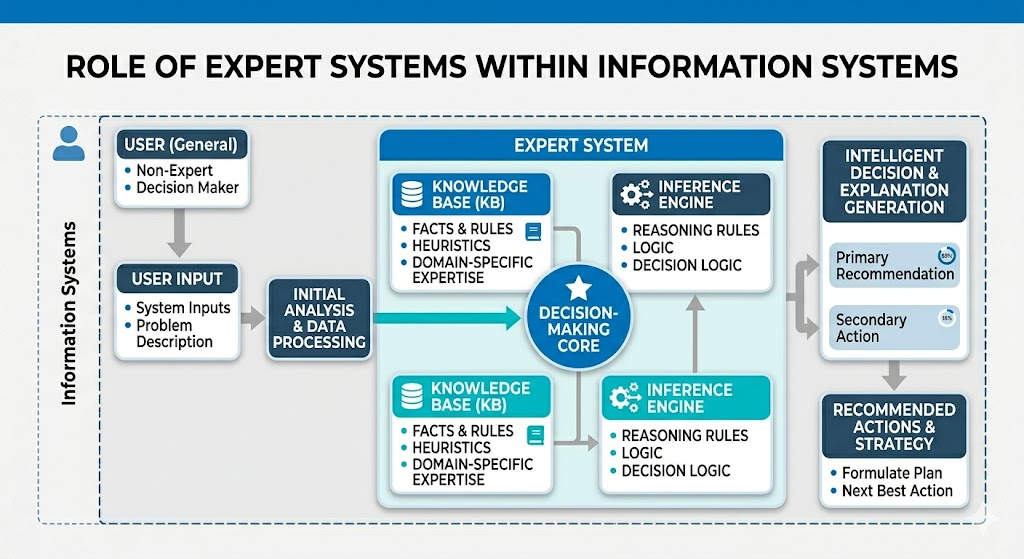
\includegraphics[width=0.6\textwidth]{role_within_is.png}
\caption{Role of Expert Systems within Information Systems}
\label{fig:expert_system_role}
\end{figure}


\newpage
\section{Architecture of Expert System}

The architecture of an Expert System defines the structure and interaction of its core components that enable intelligent decision-making. These components work together to simulate the reasoning process of a human expert by processing input data, applying domain knowledge, and generating conclusions.

A typical Expert System consists of five major components: the Knowledge Base, Inference Engine, Working Memory, User Interface, and Explanation System. Each component plays a specific role in ensuring accurate and efficient problem-solving.

\begin{figure}[h]
\centering
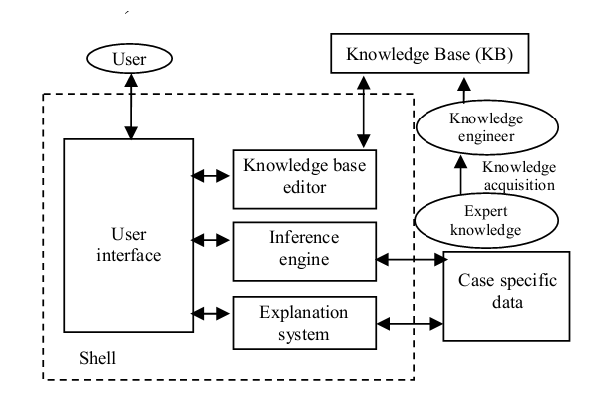
\includegraphics[width=0.7\textwidth]{general_architecture.png}
\caption{General Architecture of an Expert System}
\label{fig:expert_system_architecture}
\end{figure}

\subsection{Knowledge Base}

The Knowledge Base is the core component of an Expert System. It contains domain-specific knowledge in the form of facts and rules that represent the expertise of human specialists. The knowledge is typically structured as \textit{if-then} rules, allowing the system to apply logical reasoning.

In a medical diagnosis system, the knowledge base may include rules such as:
\begin{itemize}
    \item If a patient has high fever and cough, then there is a possibility of infection.
    \item If symptoms include chest pain and shortness of breath, then consider cardiac conditions.
\end{itemize}

The quality and completeness of the knowledge base directly influence the accuracy of the system.

\subsection{Inference Engine}

The Inference Engine is the reasoning component of the Expert System. It applies logical rules from the knowledge base to the facts stored in working memory to derive conclusions or recommendations.

There are two main reasoning strategies:
\begin{itemize}
    \item \textbf{Forward Chaining} -- Starts from known facts and applies rules to reach a conclusion.
    \item \textbf{Backward Chaining} -- Starts with a possible conclusion and works backward to verify if the conditions are satisfied.
\end{itemize}

In medical systems, forward chaining may be used to analyze symptoms, while backward chaining may be used to confirm a suspected diagnosis.

\subsection{Working Memory}

Working Memory stores temporary data such as user inputs, intermediate results, and current facts during the reasoning process. It acts as a dynamic workspace where the inference engine operates.

For example, in a medical diagnosis system, patient symptoms, test results, and medical history are stored in working memory while the system evaluates possible conditions.

\subsection{User Interface}

The User Interface allows interaction between the user and the Expert System. It enables users to input data (such as symptoms) and receive system outputs (such as diagnoses or recommendations).

A well-designed interface is essential for usability, especially in critical applications like healthcare, where clarity and ease of use are important.

\subsection{Explanation System}

The Explanation System provides transparency by explaining how the system reached a particular conclusion. It answers questions such as:
\begin{itemize}
    \item Why was this diagnosis suggested?
    \item Which rules were applied?
\end{itemize}

This feature increases user trust and helps validate the system’s reasoning, particularly in domains like medicine where accountability is crucial.


\newpage
\section{Real-World Case Study: Expert System in Medical Diagnosis}

To understand how Expert Systems function in real-world applications, this section examines a medical diagnosis system inspired by early systems such as MYCIN. These systems are designed to assist healthcare professionals by analyzing patient data and providing diagnostic recommendations based on predefined medical knowledge.

\subsection{Overview of the Medical Diagnosis System}

A medical Expert System takes patient-related inputs such as symptoms, medical history, and test results, and processes this information using a knowledge base of medical rules. The system then generates possible diagnoses and suggests appropriate treatments.

Such systems are widely used as Clinical Decision Support Systems (CDSS), helping doctors make informed decisions, especially in complex or time-critical situations.

\begin{figure}[h]
\centering
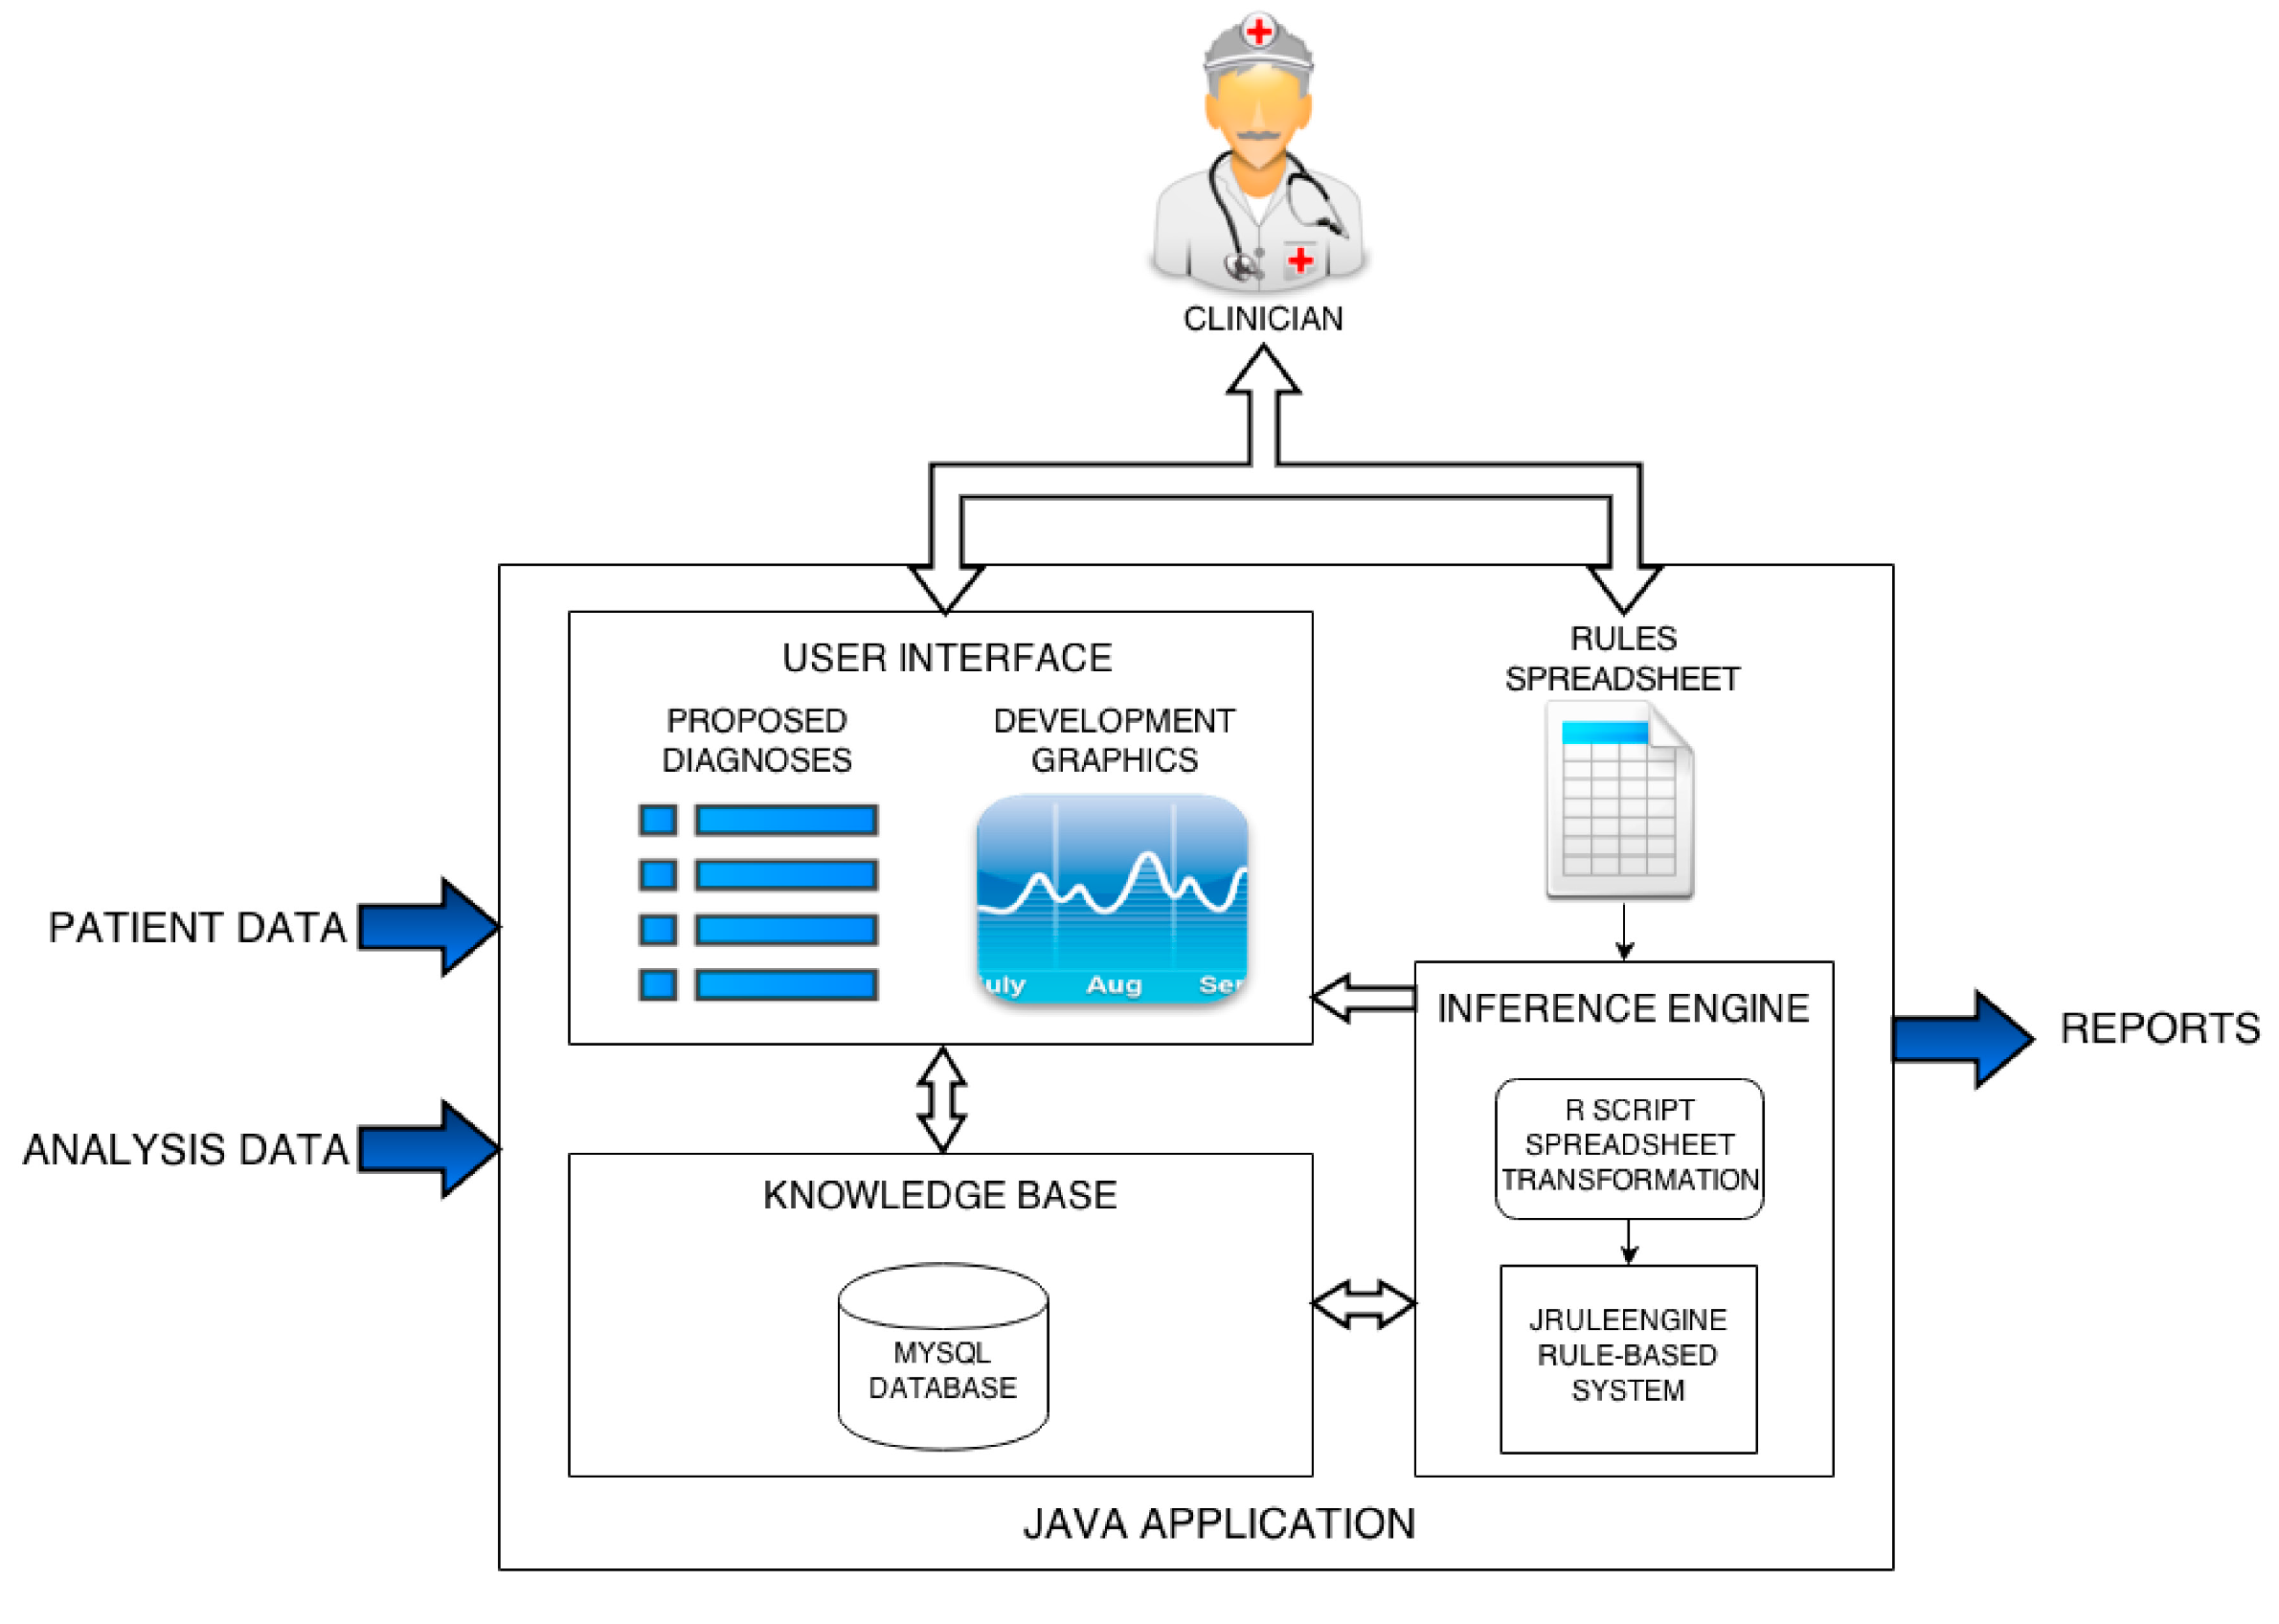
\includegraphics[width=0.7\textwidth]{medical_diagnosis_expert_system.png}
\caption{Medical Diagnosis Expert System Workflow}
\label{fig:medical_system_workflow}
\end{figure}

\subsection{Mapping Expert System Components to Medical Diagnosis}

The architecture of the Expert System can be directly mapped to its functionality in a medical diagnosis scenario:

\begin{itemize}
    \item \textbf{Knowledge Base} -- Contains medical knowledge such as disease symptoms, diagnostic rules, and treatment guidelines. For example, rules linking symptoms like fever, cough, and fatigue to possible infections.

    \item \textbf{Inference Engine} -- Processes patient data and applies medical rules to infer possible diagnoses. It evaluates combinations of symptoms and determines the most likely condition.

    \item \textbf{Working Memory} -- Stores patient-specific data including current symptoms, test results, and medical history during the diagnostic process.

    \item \textbf{User Interface} -- Allows doctors or healthcare staff to input patient information and receive diagnostic suggestions and recommendations.

    \item \textbf{Explanation System} -- Provides reasoning behind the diagnosis, explaining which symptoms and rules led to the conclusion.
\end{itemize}

\subsection{Step-by-Step Diagnostic Process}

The operation of the system can be described in the following steps:

\begin{enumerate}
    \item The user inputs patient data such as symptoms (e.g., fever, cough, chest pain).
    
    \item The data is stored in working memory for processing.
    
    \item The inference engine applies rules from the knowledge base using forward or backward chaining.
    
    \item The system evaluates possible conditions and identifies the most probable diagnosis.
    
    \item The system presents the diagnosis along with recommended actions or treatments.
    
    \item The explanation system provides justification for the decision, increasing transparency and trust.
\end{enumerate}

\newpage
\section{Intelligent Systems}

Intelligent Systems represent an advanced form of artificial intelligence that extends beyond the rule-based reasoning of traditional Expert Systems. While Expert Systems rely on predefined knowledge and logical rules, Intelligent Systems incorporate learning, adaptability, and data-driven decision-making capabilities.

These systems are designed to analyze large volumes of data, identify patterns, and improve their performance over time without explicit reprogramming. By leveraging technologies such as machine learning, neural networks, and data analytics, Intelligent Systems can operate effectively in dynamic and complex environments.
\begin{figure}[h]
\centering
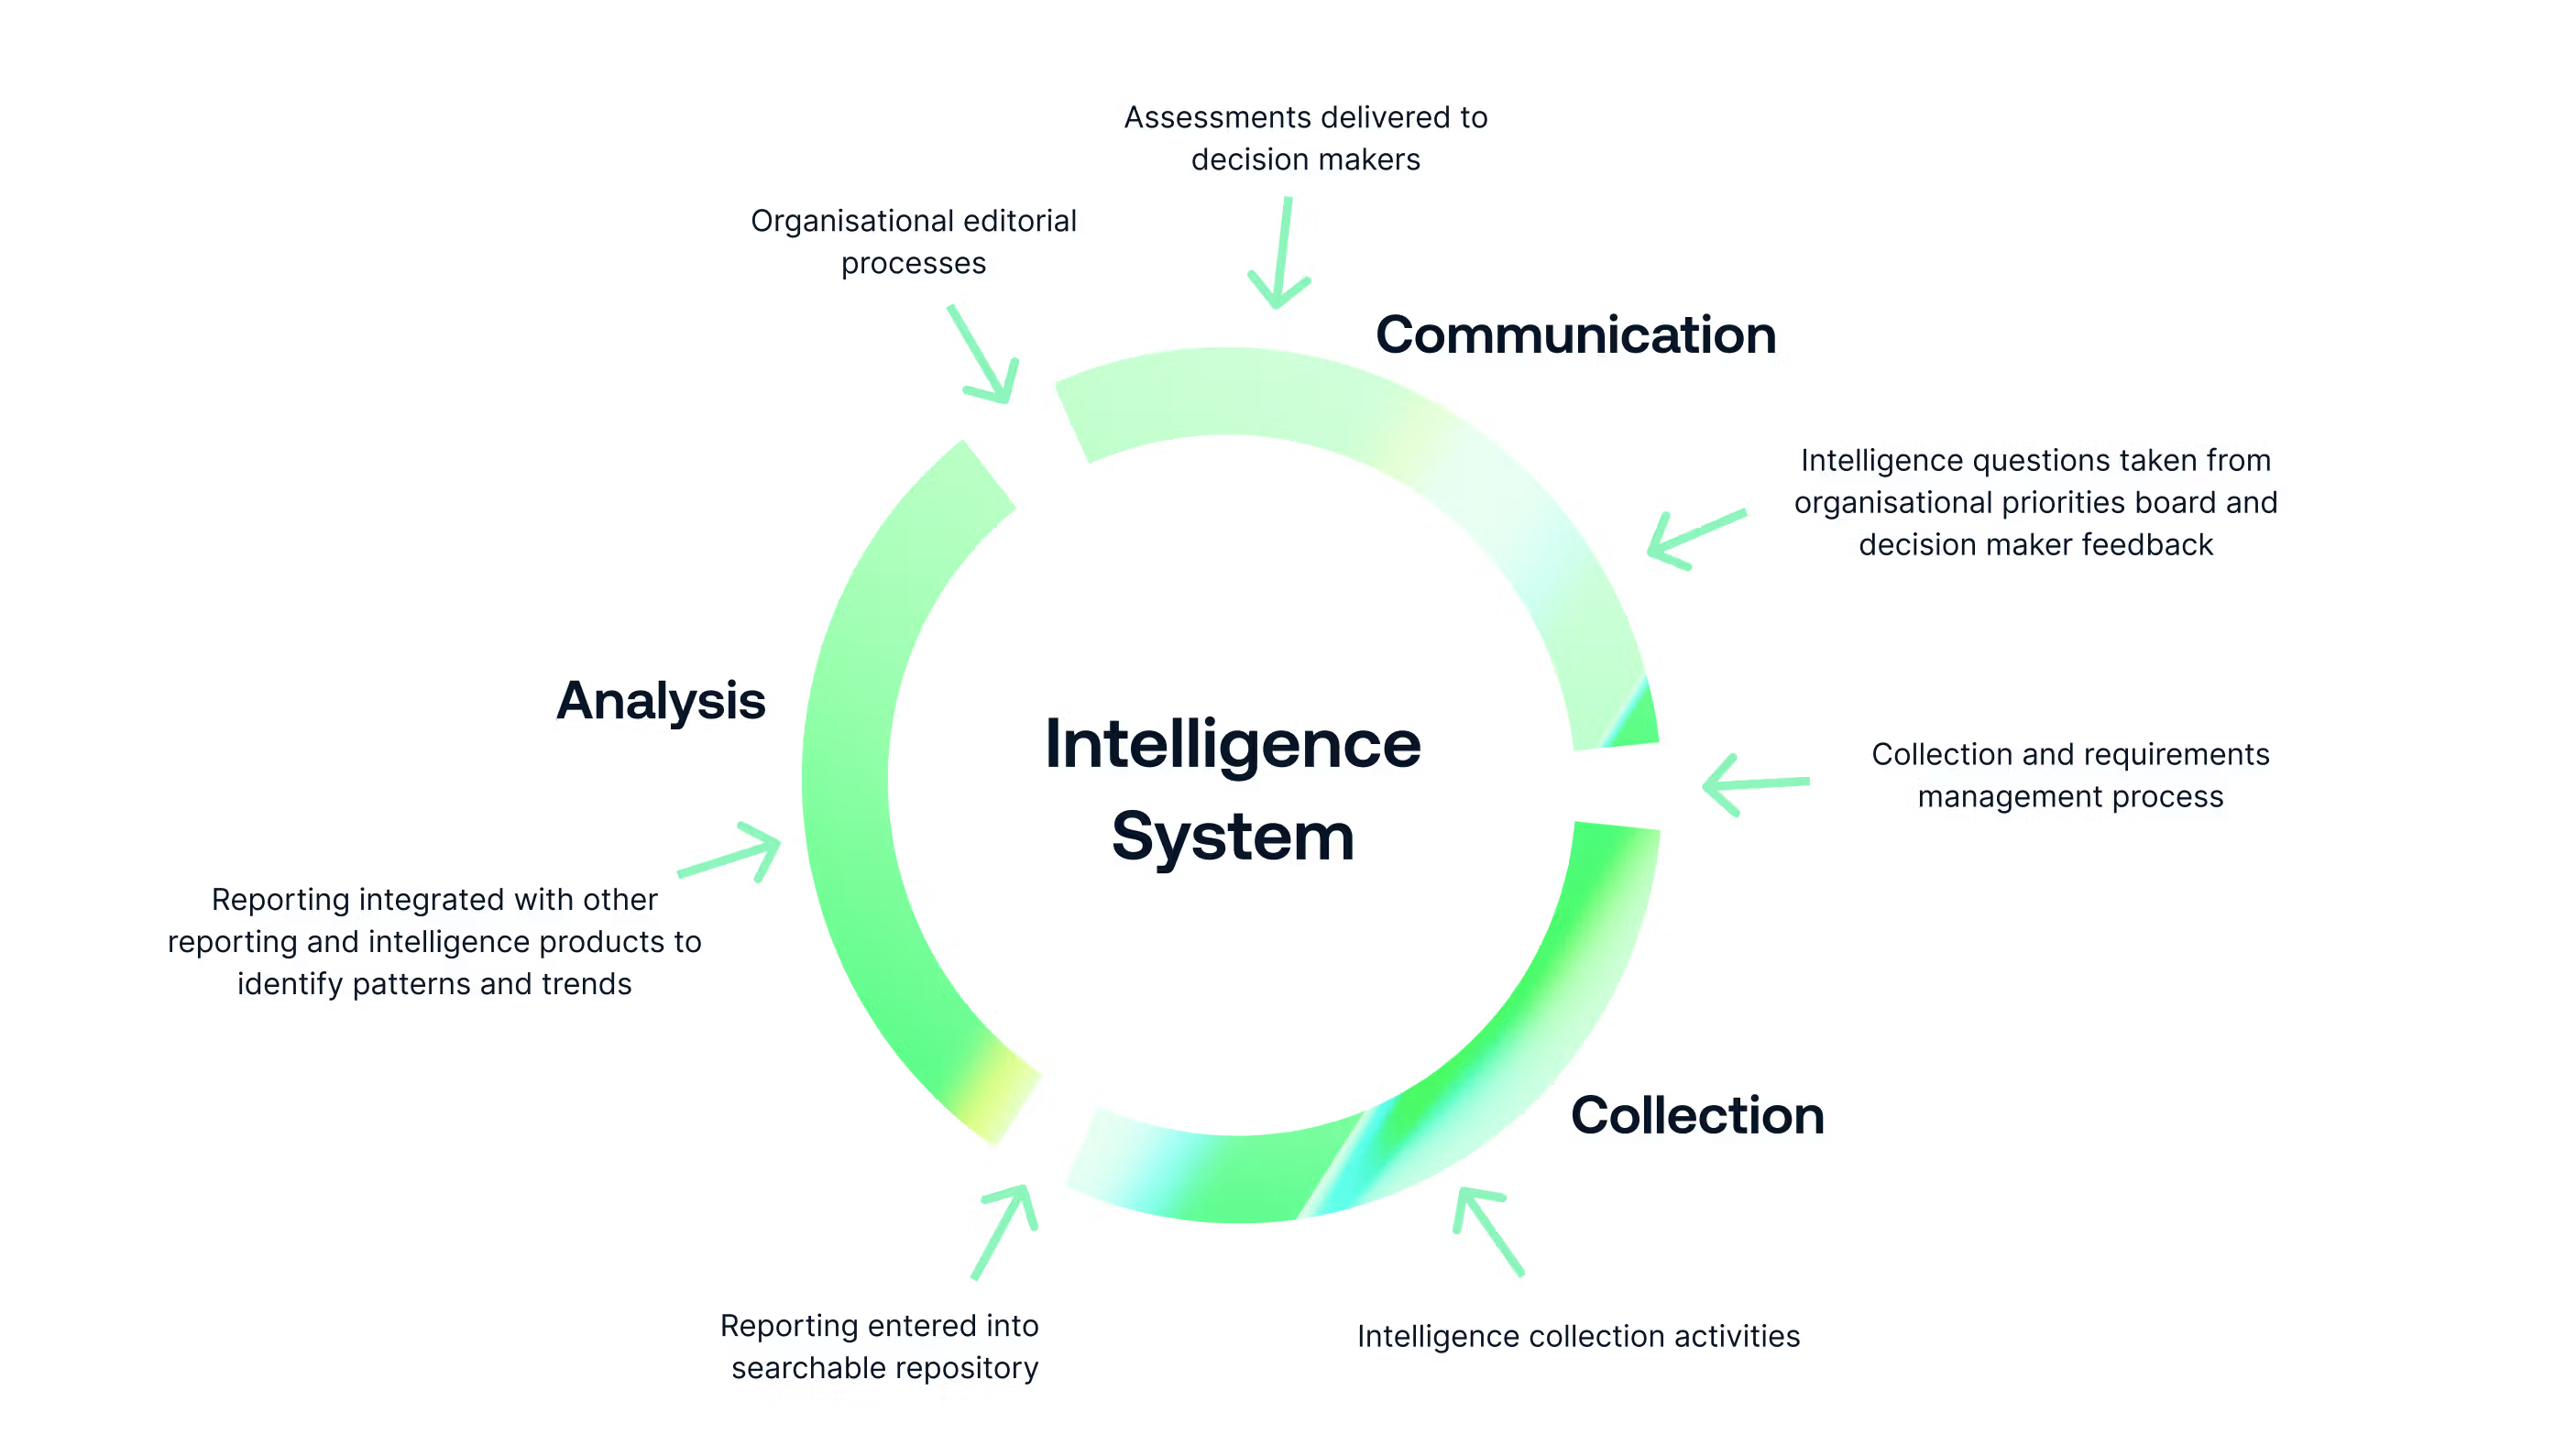
\includegraphics[width=0.7\textwidth]{intelligent_system.png}
\caption{Intelligent System}
\label{fig:intelligent_system}
\end{figure}



\subsection{Key Characteristics of Intelligent Systems}

Intelligent Systems exhibit several defining features:

\begin{itemize}
    \item \textbf{Learning Capability} -- They can learn from historical data and improve their performance over time.
    
    \item \textbf{Adaptability} -- They adjust to new data, changing conditions, and evolving environments.
    
    \item \textbf{Pattern Recognition} -- They identify hidden patterns and relationships within large datasets.
    
    \item \textbf{Autonomous Decision-Making} -- They can make decisions with minimal human intervention.
    
    \item \textbf{Scalability} -- They can handle large-scale, data-intensive applications efficiently.
\end{itemize}

\subsection{Role in Information Systems}

In modern Information Systems, Intelligent Systems enhance traditional functionalities by enabling predictive analytics, automation, and real-time decision-making. They transform static systems into dynamic platforms capable of continuous improvement and intelligent behavior.

For example, in healthcare systems, Intelligent Systems can analyze large datasets of patient records to predict disease risks, recommend personalized treatments, and support early diagnosis. Unlike Expert Systems, which depend on predefined rules, Intelligent Systems can discover new insights from data that may not be explicitly encoded.

\subsection{Examples of Intelligent Systems}

Common examples of Intelligent Systems include:

\begin{itemize}
    \item \textbf{Machine Learning Models} -- Used for prediction, classification, and anomaly detection.
    
    \item \textbf{Neural Networks} -- Applied in image recognition, speech processing, and medical imaging analysis.
    
    \item \textbf{Recommendation Systems} -- Used in platforms like e-commerce and streaming services to suggest relevant content.
    
    \item \textbf{Predictive Analytics Systems} -- Used in healthcare, finance, and marketing to forecast future outcomes.
\end{itemize}

\newpage
\section{Benefits and Future Impact}

Expert Systems and Intelligent Systems have significantly enhanced the capabilities of modern Information Systems by improving decision-making, efficiency, and scalability. As technology continues to evolve, these systems are expected to play an increasingly important role across various industries.

\subsection{Benefits of Expert Systems}

Expert Systems provide several advantages, particularly in structured and knowledge-driven domains:

\begin{itemize}
    \item \textbf{Improved Decision Accuracy} -- By utilizing expert-level knowledge and logical reasoning, these systems reduce human error and provide reliable recommendations.
    
    \item \textbf{Consistency in Decision-Making} -- Expert Systems produce consistent results for similar inputs, ensuring standardized outcomes.
    
    \item \textbf{Knowledge Preservation} -- They capture and store expert knowledge, preventing the loss of expertise due to retirement or workforce changes.
    
    \item \textbf{Time Efficiency} -- They enable faster decision-making, especially in time-critical environments such as healthcare.
    
    \item \textbf{Decision Support} -- They assist professionals by providing guidance rather than replacing human judgment.
\end{itemize}

\subsection{Benefits of Intelligent Systems}

Intelligent Systems extend these advantages by incorporating learning and adaptability:

\begin{itemize}
    \item \textbf{Continuous Learning} -- They improve performance over time by learning from new data.
    
    \item \textbf{Handling Complex Data} -- They can process large-scale and unstructured data such as images, text, and sensor data.
    
    \item \textbf{Predictive Capabilities} -- They enable forecasting and early detection of potential issues, such as disease prediction in healthcare.
    
    \item \textbf{Automation} -- They reduce manual effort by automating repetitive and complex tasks.
    
    \item \textbf{Scalability} -- They can operate efficiently in large and dynamic environments.
\end{itemize}

\subsection{Future Impact on Information Systems}

The integration of Expert Systems and Intelligent Systems is expected to transform traditional Information Systems into intelligent, autonomous, and adaptive platforms. Several key trends highlight their future impact:

\begin{itemize}
    \item \textbf{Smart Healthcare Systems} -- Advanced diagnostic tools combining rule-based reasoning and machine learning will improve patient care and early disease detection.
    
    \item \textbf{Autonomous Decision-Making} -- Systems will increasingly make independent decisions in areas such as finance, logistics, and smart infrastructure.
    
    \item \textbf{Integration with Big Data and IoT} -- Intelligent Systems will analyze data from connected devices to provide real-time insights and predictions.
    
    \item \textbf{Explainable AI} -- Future systems will focus on transparency, combining the explainability of Expert Systems with the power of machine learning.
    
    \item \textbf{Human-AI Collaboration} -- These systems will act as intelligent assistants, enhancing human capabilities rather than replacing them.
\end{itemize}

\subsection{Overall Evaluation}

Expert Systems and Intelligent Systems are not only beneficial but essential for the future of Information Systems. While Expert Systems provide structured, reliable, and explainable decision support, Intelligent Systems offer adaptability, learning, and scalability.

Together, they form the foundation of next-generation intelligent systems that will drive innovation across industries, particularly in healthcare, where accurate and timely decisions can have a significant impact on human lives.


\newpage
\section{Conclusion}

The evolution of Information Systems has been significantly influenced by the integration of artificial intelligence technologies, particularly Expert Systems and Intelligent Systems. Traditional systems, which primarily focused on data storage and processing, have transformed into intelligent platforms capable of supporting complex decision-making processes.

This case study examined the architecture of Expert Systems and demonstrated how their core components—knowledge base, inference engine, working memory, user interface, and explanation system—work together to simulate human expertise. Through the real-world example of a medical diagnosis system, it was shown how these systems can effectively assist professionals by providing accurate, consistent, and explainable recommendations.

Furthermore, the study explored Intelligent Systems as an advancement over traditional Expert Systems. By incorporating learning capabilities, adaptability, and data-driven approaches, Intelligent Systems address the limitations of rule-based systems and enable more flexible and scalable solutions. The comparison between the two highlighted their complementary strengths, suggesting that their integration can lead to more powerful and efficient Information Systems.

The benefits and future impact of these systems indicate that they will continue to play a critical role across industries, particularly in healthcare, where decision accuracy and timeliness are essential. The combination of rule-based reasoning and machine learning is expected to drive the development of intelligent, autonomous, and explainable systems.

In conclusion, Expert Systems and Intelligent Systems are fundamental to the advancement of modern Information Systems. Their continued development and integration will shape the future of technology by enhancing human decision-making, improving efficiency, and enabling innovative solutions to complex real-world problems.


\end{document}